% !TeX root = ./thesis.tex










%==============================
\chapter{Bird Flocks}
\label{ch:birdFlocks}


%-----
\section{Flock Formations}
Of all coordinated groups of moving vertebrates, birds are at the same time the easiest to observe and perhaps the most difficult to study \cite{heppner:1997}. This is primarily because most of the animal congregation research is highly dependent on collecting \cite{heppner:1997,jaffe:1997} large sets of four-dimensional data (\ie\ three in space and one in time). In fact, as a contrast to birds, most mammals move in a two-dimensional plane, which simplifies obtaining real-world data, and fish can be brought into a laboratory and enclosed in an aquarium for study. Probably because of the easier and more fruitful tracking of confined objects \cite{heppner:1997,parrish:1997a}, fish schools have been a frequent research theme \cite{aoki:1982,dill:1997,mcfarland:1997,partridge:1982,shaw:1962,terzopoulos:1994,tu:1994,tu:1999,ward:2001,zaera:1996}. 

On the other hand, scientists involved in bird congregations research are challenged by the highly difficult and almost luck-dependent data collection \cite{heppner:1997}. Just the fact that a single bird in an organized flock can move through six degrees of freedom at velocities up to 150 km/h makes collecting real-world data very difficult. Flocks fly in a three-dimensional space that cannot be easily contained and their flight paths cannot be predicted. Even by knowing the locations where there is a reasonable probability of flock appearance one cannot predict its flight path. Furthermore the three-dimensional acquisition and analysis techniques generally demand either fixed camera or detector positions. The free-flying flocks must thus be either induced to fly in the field of the cameras or the cameras must be placed in locations where there is reasonable probability that adventitious flocks will move through their field. The difficulty of data acquisition is evident even from the existing literature \cite{gould:1974,heppner:1997,jaffe:1997,moyle:1998}. According to Heppner \cite{heppner:1997}, this may be one of the reasons why there is a current of imaginative speculation, and lively controversy in literature on bird congregation structure and internal dynamics, but little data. However, regardless of the difficulty of data acquisition, some basic understanding of bird flocks is already available. 

Birds can fly in disorganized groups, such as gulls orbiting over a landfill, or organized groups, such as the vees of waterfowl. To the evolutionist, behaviourist, or ecologist, any group is of interest, but nevertheless organized groups raise most questions. In his pioneering work from 1974 Heppner \cite{heppner:1974a} presented the first definitions of the two groups. 

\begin{definition}
	\label{def:aggregation}
	A disorganized group of birds or \emph{flight aggregation} is a group of flying birds lacking coordination in turning, spacing, velocity, flight direction of individual birds and time of take-off or landing, assembled in a given area.
\end{definition}

\begin{definition}
	\label{def:flock}
	An organized group of birds or \emph{flight flock} is a group of flying birds, coordinated in one or more of the following parameters of flight: turning, spacing, velocity, and flight direction of individual birds, and time of take-off and landing.  
\end{definition}

In this study Heppner also presented a classification of flight flock formations and a discussion of the leading research directions.\footnote{In this dissertation I primarily consider groups of birds in flight and thus will be concerned neither with their take-off nor landing. For reasons of clarity the term flight in flight flock and flight aggregation will therefore be omitted.} According to his study, there are two major classes of flight formations: \emph{line formations} and \emph{cluster formations}. Their characteristics had and still have a substantial influence on the leading research directions. Today \cite{heppner:1997,parrish:1997a}, as it was then \cite{heppner:1974a}, the examination of bird flocks is still led by two primary questions. The first, usually expressed while observing a skein of geese flying overhead, is ``\emph{Why do they fly in such a precise alignment?}'' The second comes to mind when we observe 5000 European Starlings, \emph{Sturnus vulgaris}, turning and wheeling over a roost. We ask ourselves ``\emph{How do they achieve such coordination and polarity?}'' The question `why' is thus usually expressed in reference to relatively large birds, like waterfowl, flying in line formations, whereas the question `how' is in reference to relatively large flocks of small birds, like sandpipers, flying in cluster formations. 

%--
\subsection{Line Formations}
Line formations (\fig~\ref{fig:lineFormations}) are groups of relatively large birds, such as waterfowl and pelicans, flying in a single line, or joined single lines. Typically they are approximately two-dimensional and show a rather high degree of regularity in spacing and alignment. In line formations birds fly in a single line, one behind the other (\emph{column}), one beside the other (\emph{front}) or staggered stepwise from the bird at the head of the formation (\emph{echelon}). In nature left and right echelons can be found and frequently a left echelon becomes a right echelon, and vice versa. However, the transition is not a swing from side to side, but rather a temporary breakup of the formation. In line formations birds also fly in joined single lines; left and right echelons joined at the tip of the formation (\emph{`J'} and \emph{`V'}) or at the tail of the formation (\emph{inverted `J'} and \emph{inverted `V'}). In the `V' and inverted `V' formation the left and right echelon are approximately the same size, whereas in the `J' and inverted `J' formation one is considerably larger.

\begin{figure}
	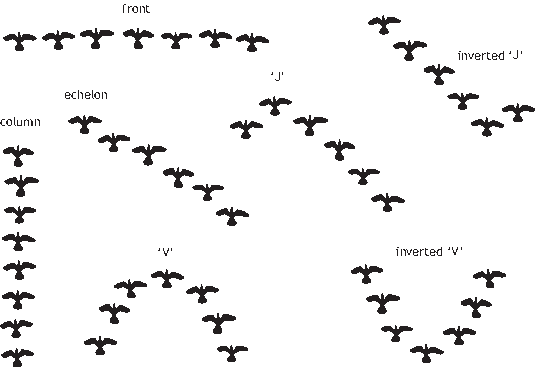
\includegraphics{fig_lineFormations}
	\caption{Line formations: column, front, echelon, `J', `V', inverted `J', and inverted `V' \cite{heppner:1974a}.}
	\label{fig:lineFormations}
\end{figure}

%--
\subsection{Cluster Formations}
Cluster formations (\fig~\ref{fig:clusterFormations}) are relatively large flocks of small birds, like sandpipers, characterized by development in the third dimension, and rapid, apparently synchronous turns. In cluster formations birds are typically distributed over a three-dimensional space of an irregular spheroidal shape that is, when observed perpendicularly to the plane of flight: as wide as it is long (\emph{globular cluster}), wider than it is longer (\emph{front cluster}), or longer than it is wider (\emph{extended cluster}). Birds flying in globular clusters generally fly in apparent close order and can be seen making very rapid turns. Similarly, front clusters tend to have very precise spacing and turning. The front cluster is often seen in pigeons. However, birds flying in extended clusters tend to be rather disorganized, with frequent breakoffs and shifts of position. This formation may simply be a disorganized group of birds that happen to be flying independently toward a common destination (\ie\ an aggregation) \cite{heppner:1974a}.

\begin{figure}
	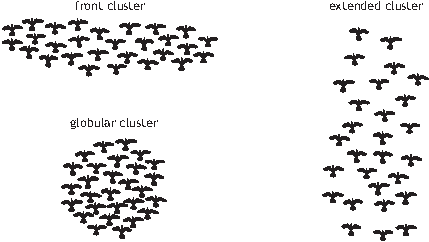
\includegraphics{fig_clusterFormations}
	\caption{Cluster formations: front cluster, globular cluster, and extended cluster \cite{heppner:1974a}.}
	\label{fig:clusterFormations}
\end{figure}


%-----
\section{Simulating Bird Flocks}
While observing line formations, one is impressed by the precision with which relatively small numbers of large birds maintain themselves in accurate spatial alignment and angular orientation with their flockmates. On the other hand, while observing cluster formations, the attention is drawn to the coordination that enables large numbers of small birds, flying in close order, to wheel and turn without suffering mid-air collisions. In the first case the primary interest is the functional significance of formation flight \cite{heppner:1997,speakman:1998}. In the second the attention is given to the synchrony, or apparent synchrony, in the turning movements and the necessity or presence of a leader guiding these manoeuvres.

In the mid 1980s different papers appeared, suggesting that coordination in cluster flocks might be achieved by the application of the mathematics of nonlinear dynamics \cite{okubo:1986} and that flocking might be an emergent property arising from individuals following simple rules of movement \cite{heppner:1987}. At the same time, but working in another field of study, namely computer graphics, Reynolds \cite{reynolds:1987} published a ground-breaking seminal paper that first presented a computer model of bird flocking. His primary objective was a believable animation of a bird flock. In his study a collection of individuals whose behaviour is governed by three simple rules based on geometrical calculations, demonstrates flocking behaviour that is typical for flying birds. Without knowing about Reynolds's work, ornithologist Frank Heppner joined forces with mathematician Ulf Grenander and published the second computer model of bird flocking \cite{heppner:1990}. In their model the flock was a self-organizing collection of individuals, whose behaviour was based on stochastic nonlinear differential equations. Nevertheless, both models base their assumptions on common grounds and model the behaviour of individuals on the, at times contradictory, clues of attraction and repulsion. The mutual coexistence and importance for the congregation's structure of these two clues was already suggested by Okubo \cite{okubo:1980}.

After 1990 papers regarding computer models of bird flocking subsided. The rare exceptions were the studies of the evolution of flocking behaviour \cite{reynolds:1993a,reynolds:1993b,reynolds:1994,spector:2002,spector:2003} and Heppner's unpublished study of flock take-off and landing \cite{heppner:1997}. In the last few years the field has been slowly regaining scientific interest. Recent research, however, builds on the two original models. Tanner, Jadbabaie, and Pappas \cite{tanner:2003a,tanner:2003b} for example concentrate on the stability analysis of an organized flock that is based on Reynolds's model. Couzin \etal\ \cite{couzin:2005}, on the other hand, employ Reynolds's model to examine leadership and decision making in animal groups on the move. Their approach adds a preferred flight direction only to a proportion of the modelled digital birds. Their study reveals that the larger the group the smaller the proportion of informed individuals needed to guide the group, and that only a small proportion is required to achieve great accuracy. A rare example of a different, and also the most recent, approach is that of Wiltschko and Nehmzow \cite{wiltschko:2005}, but its primary concern is not flocking but rather the navigation process employed by pigeons. 

The primary reasons for the loss of research interest may lie hidden in the mathematical nature of these simulations as well as in the amount of work that is required to master the effects that parameter changes have on the displayed behaviour. Even Heppner and Grenander \cite{heppner:1990} admit that the interesting patterns were discovered serendipitously and that considerable trial-and-error experimentation was needed before flock-like behaviour was produced.

In addition, one can hardly imagine that flocking birds flying at speeds up to 150\,km/h \cite{heppner:1997} have the time or the ability to perform sophisticated or time-intensive mathematical calculations. Even Parrish \etal\ \cite{parrish:1997a} state that there must be simple traffic rules for species' engaging in collective movement. To continue, considering our perception of the surrounding environment, it is difficult to imagine that birds are able to perceive precise (\ie\ crisp) information (\eg\ distance). However, all of the existing mathematical models assume such capabilities.

Furthermore, the mathematical nature of the existing models means that a substantial mathematical understanding was required for their construction as is required for their thorough understanding. In my opinion this represents a major drawback for their usability. The mathematical nature, if truth be told, makes the models difficult to understand by the audience they were designed for. The latter is predominantly composed of ethologists, not mathematicians. Even if one makes the models as black-box modules and allows only changing the values of parameters, this would not suffice for truth-testing. Truth-testing any sort of simulation that purports to represent natural behaviour is extremely difficult, and has not often been done, especially in behaviour. Models are usually too crude, or have too many special conditions to be readily tested with real-world data. This is probably why ethologists have difficulties in using the models for testing the existing hypotheses or forming new ones.

%--
\subsection{Computer Model by Craig W. Reynolds}
\label{subsec:birdFlocks:cwr}
Traditionally an animator who wanted to animate a bird flock would carefully set up numerous key frames that defined the motion paths of every single flock member. When animating a line flock, especially if it is a very small one, such an approach is somehow possible. Difficulties arise when large cluster flocks are being animated. In this case animating each and every flock member becomes painstaking and tedious, and is, disregarding the difficulty of corrections, without inter-bird collisions almost impossible to do. 

As already mentioned, Craig W. Reynolds, in his pioneering work from 1987, presented the first computer model of bird flocking \cite{reynolds:1987}. When reflecting on how to animate a bird flock he treated the latter as any group of entities that exhibit the general class of aligned, noncolliding, aggregate motion. This means that with the term flock Reynolds refers also to schools, herds, \etc\ However, when speaking about bird flocks it can be seen that his notion is more strict than definition~\ref{def:flock}. In fact, he assumes an organized flock to be coordinated in all of the flight parameters as well as that there are no collisions. However, the requirements of definition~\ref{def:flock} are met also when coordination is only in some of the parameters of flight and the definition does not make note of the absence of collisions. The latter on one hand seems plausible, however, on the other hand, especially in large cluster flocks, because of their size, the relatively small inter-bird spacing and fast manoeuvres, seems almost impossible.

In the mid 1980s the decentralization ideology \cite{resnick:1997} was becoming ever more influential. This was also the time when the research field of \emph{artificial life} \cite{adami:1998,emmenche:1994,langton:1989} was emerging. Both, together with Reynolds's prior work \cite{reynolds:1978,reynolds:1982}, led him toward the idea that a flock of birds, as perceived by one of its members, is something completely different than as perceived by an outside observer. It is much like the difference between driving in traffic and standing on a roadside watching traffic whiz by. This represented an important step forward. He did not look at the flock as a whole any more or searched for a single rule that describes it---known as \emph{top-down approach}. On the contrary, he imagined what it would be like to be a member of the flock and searched for the rules to follow in order to stay in the flock---known as the \emph{bottom-up approach}. This approach is characteristic for modelling artificial life \cite{adami:1998,emmenche:1994,gardner:1970,langton:1984,langton:1989,rucker:1993,terzopoulos:1994,terzopoulos:1999,tu:1999,ward:2001}. I am talking about modelling by constructing a large number of primary entities, whose local interactions base on simple rules, and observing the emergent global behaviour, behaviour not previously programmed according to specific rules \cite{emmenche:1994}. Later, in computer graphics, Reynolds's approach, when one actually seeks to model the behaviour of an object and not its shape or physical properties,  became known as \emph{behavioural animation} \cite{reynolds:1987}.

Reynolds \cite{reynolds:1987} came to the conclusion that as a member of a flock he would have to successfully coordinate three different drives. He found out that, in order to fly without collisions, he would have to make sure that he was not too close to any of his flockmates. In other words, he would try to maintain a certain separation distance. Furthermore, he would have to try to fly with the same flight speed and in the same flight direction as his flockmates. This also means that it would be highly unlikely that he collided with them in the near future. And finally if he noticed that all of the flockmates were on one of his sides he would wish to drift towards them. Written in the form of simple rules these drives are \cite{reynolds:1987,reynolds:1999,reynolds:2000}:

\begin{itemize}
	\item {\emph{separation}}: avoid collisions with nearby flockmates,
	\item {\emph{alignment}}: attempt to match flight speed and flight direction with nearby flockmates,
	\item {\emph{cohesion}}: attempt to stay close to nearby flockmates.
\end{itemize}

The cohesion and separation drives, when viewed in unison, represent the so-called \emph{attraction-repulsion} scheme \cite{okubo:1980}. The alignment drive, on the other hand, is used to produce \emph{polarization}, which is another important feature of animal groups of uniform density \cite{parrish:1997a}. 

Reynolds translated the three drives to a set of geometrical equations, where he interpreted the expression `nearby flockmates' as the bird's immediate surroundings (see subsection~\ref{subsec:birdFlocks:cwr}). Actually, he found out that a bird does not require full knowledge about the positions, flight speed and flight direction of every bird in the flock, but only a small subset. The expression `nearby flockmates' thus addresses the bird's awareness of another bird and Reynolds based its computation on the distance and direction of the offset vector between them. His digital bird\footnote{Actually Reynolds refers to the digital (simulated) bird-like, ``bird-oid'' objects, generically as \emph{boids} even when they represent other sorts of creatures such as schooling fish \cite{reynolds:1987}.} thus actually has a localized perception of the world with a certain distance and field of view and can be visualized as a perception volume shaped like a sphere with a cone removed from the back. It is important to note that, when the digital birds are in a flock, the individual perception volumes overlap and each individual bird will probably end up in a number of perception volumes.

With a limited perception volume, Reynolds makes a very good point stating that a bird's perception of the world is severely limited by occlusion (\ie\ nearby birds hide those far away), but inside the perception volume he does not take this into account. Furthermore, even though he limits the digital bird's awareness of the world, the perceived information is accurate, meaning that the digital bird has full and precise knowledge about the position, flight speed and flight direction of its flockmates. In my opinion this approach is still defective. It is true that Reynolds does not try to model visual perception but tries to make available approximately the same information that is available to a bird as the end result of perceptual and cognitive processes. However, all of the obtained information is still based on visually perceptible information. A bird's visual perception is not limited only by occlusion, but also by the fact that the ability to sense distance, apart from being affected by the degree of binocular overlap, decreases with distance itself. Moreover, in his latest implementation of the model,\footnote{OpenSteer v0.8, \href{http://opensteer.sourceforge.net/}{http://opensteer.sourceforge.net/}.} Reynolds uses three distinct perception volumes, one per drive. According to my experiments (see \chaptername~\ref{ch:analysis}) this introduces unwanted `unnatural' behaviour.

Furthermore, Reynolds models the cohesion drive as the digital bird's tendency to fly toward the centre of mass of the nearby flockmates. I find this somewhat questionable. The centre of mass is a mathematical construct and it is difficult to believe that a real bird has knowledge of such constructs or uses them to compute its action. It is true that it was Pliny \cite{heppner:1997} who noted that ``it is a peculiarity of the starling kind that they fly in flocks and wheel round in a sort of circular ball, all making towards the centre of the flock''. However, in my opinion, real birds might not have any idea about the centre of the flock and their making towards it might be just an emergent property by itself.

In Reynolds's approach an individual digital bird thus, based on the precise information about the position, flight speed and flight direction of its flockmates, using geometrical equations, computes the three desired changes of flight direction and flight speed, each satisfying one drive. As Reynolds models the digital bird as a point mass (simple) vehicle \cite{reynolds:1987,reynolds:1999}, he represents the desired change in flight direction and flight speed as the physical force that would induce it. The digital bird thus computes the actual change in flight direction and flight speed by computing a weighted sum of the resulting three physical forces (see subsection~\ref{subsec:animat:cwr} for more detail).
 
%--
\subsection{Computer Model by Frank H. Heppner and Ulf Grenander}
\label{subsec:birdFlocks:fhh}
As a contrast to animators who try to produce a flock animation that visually resembles a natural flock in a way that could take in a theatre spectator, flocks interest ornithologists from a completely different point of view. The synchrony, or apparent synchrony, in the turning movements of cluster flocks has drawn much attention from ornithologists. The key research directions were, and still are, guided mostly by the question how flocks coordinate their movement and decide when to wheel or turn. With respect to this in most investigations the leading role was played by the search for evidence that would answer the question of existence or necessity of a flock leader. Indeed, many researchers assumed a leader's existence and presumed it directed the movement of the whole flock \cite{heppner:1990}. This approach was also taken by Heppner and Hafner \cite{heppner:1974b}, but they proceeded to demonstrate the formidable obstacles to visual or acoustic communication between such a putative leader and its followers. Nevertheless, efforts to identify the flock's leader have been so far unsuccessful, even when using methods that permit an analysis of the position of individually identified birds in a free-flying pigeon flock \cite{pomeroy:1992}. In the meantime reports appeared \cite{davis:1980} which suggested that the coordinated turning might be an emergent phenomenon; the result of individual birds `voting' with their bodies on the flight path the flock should take. According to this theory the flock turns in the direction expressed by the initiators only when a `critical mass' is reached. Recently, a similar approach has been used by Couzin \etal\ \cite{couzin:2005} to examine leadership and decision making in animal groups on the move.

Similar to Reynolds, ornithologist Frank H. Heppner started pondering the idea that flocks might be an emergent phenomenon; the result of a group of individuals following simple rules. This idea was, again as in Reynolds's case, initially inspired by artificial life research; by Conway's `Game of Life' \cite{gardner:1970}, to be more precise. Moreover, also by the emerging suggestions that coordination in cluster flocks could be achieved by the application of nonlinear dynamics \cite{okubo:1986}. As ornithologists in most cases are not mathematicians, Heppner joined forces with applied mathematician Ulf Grenander, to translate his ideas into mathematical equations. The result of their work was the second computer model of bird flocking \cite{heppner:1990} given through a stochastic differential driven by a Poisson process. As in Reynolds's case, the model developed by Heppner and Grenander also suggested that birds coordinate through three, but different drives. They assumed that the coordination in flocks emerges because birds try to accomplish the following drives:

\begin{itemize}
	\item \emph{homing}: each member of the flock tries to stay in the roosting area,

	\item \emph{velocity regulation}: each member of the flock tries to fly with a certain predefined flight speed---it tries to return to that speed if perturbed,
	
	\item \emph{interaction}: if two flockmates are too close to one another, they try to move apart; if they are too distant, they do not influence each other; otherwise they try to move closer together. 
\end{itemize}

As already said, Grenander translated these drives into mathematical equations that depended on the current position of the digital bird (homing), its flight speed (velocity regulation) or its distance from other digital birds (interaction). But their digital bird has complete and precise information about the locations of other digital birds. With this Heppner and Grenander make an unrealistic assumption because, as already discussed, real birds have limited and inaccurate perceptive capabilities.

As a contrast to Reynolds, who modelled the principles of attraction and repulsion in the form of two distinct drives, Heppner and Grenander combined them into one drive (interaction). Combined or not, the two drives seem reasonable and `natural', after all, their mutual coexistence and importance for the congregation's structure has already been suggested by Okubo \cite{okubo:1980}. On the other hand, the velocity regulation drive used by Heppner and Grenander seems somewhat strange. They derived this drive from aerodynamic theory; with a given power output and configuration, an aircraft will maintain a constant speed, it will return to that speed if perturbed. A real bird would not have to make a decision about this. In my opinion, this results in a questionable effect. Take, for example, a digital bird that slowed down because it was too close to one of its flockmates. It will speed up. But not because it is trying to catch up with the flock, but because it is returning to the predefined preferred flight speed. In my opinion this behaviour resembles more to an aggregation of birds that happen to be flying together than to a flock of birds that are trying to fly together. Furthermore, it is hard to grasp that a bird has a predefined preferred flight speed. Even if it does, this cannot be constant in time. Even though birds (especially in line flocks) tend to fly in relatively straight lines and at very consistent speeds, they tend to change their flight speed regardless of the speed of the flock, which might, however, be primarily caused by fatigue or other distractions (\eg\ wind gusts). 

Another important feature of flocks is alignment. Heppner and Grenander \cite{heppner:1990} did not model it specifically, but they mention that in certain cases organized flocks maintaining straight direction of flight emerged. This might be caused by the perception model they used. Their digital bird has complete and accurate information about its surroundings, which means it has full and precise knowledge about the locations of all surrounding digital birds that are closer than a predefined distance. However, in their quest for realism, Heppner and Grenander, introduced also a special influence which was intended to simulate the effects of wind gusts and random local disturbances. They modelled it using a Poisson stochastic process and state that it was of crucial importance for achieving flock-like behaviour \cite{heppner:1990}.
